\chapter{The Deadly Ignorance of Position}
\label{ch:deadly-ignorance}

\section{The Scilly Disaster}
\label{sec:opening-vignette}

The fog rolled across the Atlantic with October's weight, thick as wool. \textsc{hms} Association cut through black water, the flagship of Admiral Sir \textsc{Cloudesley Shovell}, commanding the English fleet returning from Gibraltar after months of winter cruising against the French. The fleet had been at sea for weeks. The sailors' calculations, checked and rechecked against dead reckoning and the uncertain hints the stars provided on clear nights, put them safely west of the Scilly Isles---a good margin, or so they believed. The officers felt confident enough to press on toward home.

At eight o'clock in the evening, with no warning but the sound of breakers, the rocks rose up out of the darkness. Before anyone could shout orders, \textsc{hms} Association struck the Western Rocks off Scilly with a noise like the world breaking. The flagship went down at once. Within minutes, Eagle, Romney, and Firebrand struck nearby reefs. The sea boiled white around the wrecks as the ships broke apart on stone, the men struggling in water too cold to permit survival for more than minutes. Between fourteen and twenty-two hundred men died that night---officers and ordinary sailors indistinguishable in the violence of water and rock.

By morning the cries had stopped. Bodies washed onto the black sand beaches. Among them was Shovell himself, so waterlogged that identification took hours, and was confirmed only when local women recognized his ring. The fleet that had fought the French returned home as wreckage scattered across an archipelago of rocks the commander had believed lay far behind.

The court of inquiry that followed was bitter and useless. The officers swore they had computed their position carefully. The navigators swore they had done the mathematics correctly. Nobody had committed an obvious, detectable error. And yet the fleet had been, by modern reckoning, more than \SI{40}{nm} off course in a direction that put them precisely where the rocks lay waiting. That error---that invisible, undetectable, geometrically blameless error---had killed thousands.

\section{What Is Longitude?}
\label{sec:definition}

The problem is elementary in principle, impossible in practice. The Earth is a sphere, and any position on its surface requires two coordinates: one north and south, one east and west. The first is latitude. The second is longitude.

\subsection{Latitude: The Celestial Measure}

Latitude is the angle from the equator toward the poles, measured in degrees. And here the geometry cooperates with the navigator. Stand anywhere on Earth and look toward the celestial pole---south if you are in the Southern Hemisphere, north if you are in the north. The altitude of that pole above the horizon, measured in degrees, is your latitude.

\begin{figure}[htbp]
  \centering
  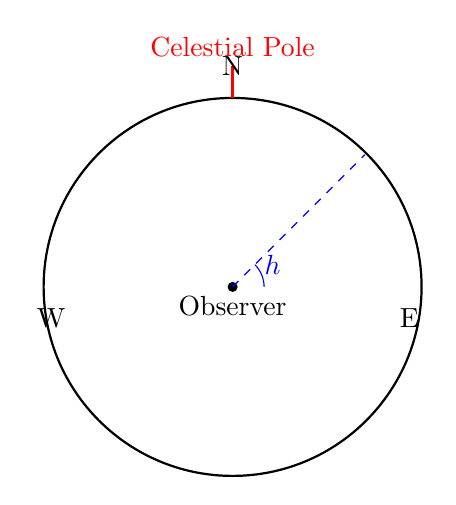
\begin{tikzpicture}[scale=0.8]
    % Horizon circle
    \draw[black, thick] (0,0) circle (3cm);
    % Celestial pole
    \draw[red, thick] (0,3) -- (0,3.5) node[above] {Celestial Pole};
    % Observer position
    \filldraw[black] (0,0) circle (2pt) node[below] {Observer};
    % Altitude angle
    \draw[blue, dashed] (0,0) -- (2.1,2.1);
    \draw[blue] (0.5,0) arc (0:45:0.5) node[right] {$h$};
    % Labels
    \node[left] at (-2.5,-0.5) {W};
    \node[right] at (2.5,-0.5) {E};
    \node[above] at (0,3.2) {N};
  \end{tikzpicture}
  \caption{Celestial pole altitude equals observer's latitude. At the equator the pole is at the horizon ($h = 0\degree$); at the North Pole it is overhead ($h = 90\degree$).}
  \label{fig:latitude-geometry}
\end{figure}

In practice, the true celestial pole is not marked by any bright star. But \emph{Polaris}, the north star, lies within one degree of it, a small enough error that a careful observation can yield latitude accurate to within a degree---the width of the full moon in the sky. Other methods exist. At noon, the Sun reaches its maximum altitude above the horizon. Measure that altitude, and know the Sun's declination (its angular distance north or south of the celestial equator) from the ephemeris, and latitude follows from simple geometry:

\[
  \phi = \delta + (90\degree - h)
\]

where $\phi$ is latitude, $\delta$ is solar declination, and $h$ is observed altitude. A careful observer with a good instrument can achieve the same degree of precision with the Sun that they achieve with Polaris.

This is the reason medieval and ancient navigators could determine latitude. The geometry of spherical astronomy cooperates. The celestial poles mark the axis of the Earth's rotation; the observer stands on a rotated coordinate system, and that system writes its angle onto the sky.

\subsection{Longitude: The Hidden Coordinate}

Longitude is the angle east or west from an arbitrary reference meridian---today the meridian passing through Greenwich, but in the seventeenth century, no single reference existed. The fundamental problem is this: longitude has no corresponding celestial marker. No star or planet sits directly over the Prime Meridian. The sky looks the same to an observer in London and an observer in Gibraltar, except for the time at which the stars rise and set.

And here is the essential insight that unlocks the whole problem: \textbf{the difference in longitude between two places equals the difference in the local time, converted to angle.}

If two observers on Earth are separated by one hour of local solar time, they stand on different meridians that are separated by $15$ degrees of longitude. This is because the Earth rotates $360$ degrees in $24$ hours, or $15$ degrees per hour. If you know the time at Greenwich, and you know your local time (which you can determine from the Sun's altitude), the difference between them, multiplied by $15$ degrees per hour, gives your longitude.

\[
  \lambda_{\text{observer}} - \lambda_{\text{reference}} = \Delta t \times \SI{15}{\degree\per\hour}
\]

But here is where the symmetry breaks: determining local time is straightforward. Determining the time at the reference meridian, while standing in the middle of the Atlantic Ocean, is not.

---

\section{The Navigator's Problem}
\label{sec:dead-reckoning}

When no absolute time reference is available, the only tool the navigator possessed was \emph{dead reckoning}---a calculation based on measured direction and estimated speed over elapsed time. It is a simple idea, and a relentlessly accumulating nightmare.

Each watch, the officer on deck estimates the ship's speed by dropping a wooden chip attached to a knotted rope into the water ahead and measuring how many knots pass through his hand in a given time (the \emph{chip log}). He notes the direction from the magnetic compass. The heading and the estimated speed are recorded in the ship's log. When summed over hours and days, these estimates become the ship's position.

\[
  \text{longitude}_{\text{new}} = \text{longitude}_{\text{old}} + \int_0^t v(\tau) \cos(\theta(\tau)) \, d\tau
\]

\[
  \text{latitude}_{\text{new}} = \text{latitude}_{\text{old}} + \int_0^t v(\tau) \sin(\theta(\tau)) \, d\tau
\]

where $v$ is estimated speed and $\theta$ is compass heading.

The mathematics is correct. The execution is catastrophic. The chip log is crude. Speed estimates may be off by $20$ percent. The magnetic compass varies in its declination (the angle between magnetic north and true north) in ways that are not fully predictable. The current is invisible and unknown. A ship sailing through fog for days accumulates errors that grow in all directions at once, magnifying and interacting.

\begin{table}[htbp]
  \centering
  \caption{Cumulative error in dead reckoning: a transatlantic crossing.}
  \label{tab:dead-reckoning-error}
  \begin{tabular}{lrr}
    \toprule
    Days at Sea & Estimated Error (nm) & Compass Direction \\
    \midrule
    5 & 10--15 & Random \\
    10 & 25--40 & Systematically westward \\
    20 & 60--100 & Westward \\
    30 & 100--150 & Westward \\
    40 (typical Atlantic) & 150--200+ & Westward \\
    \bottomrule
  \end{tabular}
\end{table}

A difference of one degree of longitude at the latitude of the English Channel corresponds to about \SI{40}{nm}---the distance between safe harbor and a reef. A crew can be in error by that much and not know it until the land appears in the wrong place, or the ship strikes rock.

---

\section{A Catalog of Disaster}
\label{sec:maritime-losses}

The Scilly disaster did not appear from nowhere. It was the culmination of a long history of wrecks and losses, each attributable to the same invisible enemy: the impossibility of knowing where you were when the horizon had vanished.

\begin{enumerate}
  \item \textbf{1591, the \textsc{São Thomé}.} Portuguese galleon en route to India struck and sank near Sumatra. The crew believed themselves to be $600$ nautical miles to the east. The ship carried $944$ people; fewer than $200$ survived. The survivors were enslaved by local peoples.
  
  \item \textbf{1615, the Eendracht.} Dutch East Indiaman, separated from her convoy, made unexpected landfall on the coast of Western Australia in the Indian Ocean's eastern reaches. The ship was lost, but the accidental discovery added a continent to European geography.
  
  \item \textbf{1656, the Tryall.} English East Indiaman struck rocks off Western Australia, also having misjudged her longitude severely. Forty men survived on a desolate island; only a handful were ever rescued.
  
  \item \textbf{1691.} A squadron of English ships, attempting to make port at Plymouth in fog, struck rocks near the English coast. Five ships lost; the incident provoked outrage.
  
  \item \textbf{1707, the Scilly Disaster.} \textsc{hms} Association, Eagle, Romney, and Firebrand, with Admiral Shovell commanding the fleet. Twenty-two hundred dead. The court of inquiry concluded that no one was obviously at fault.
\end{enumerate}

Each loss was, by the standards of the time, inexplicable and blameless. The officers had followed procedures. The calculations had been correct. The instruments had been as good as the age could provide. And yet the ships had gone down anyway, leaving the maritime powers of Europe staring at a problem that appeared to be unsolvable with the tools at hand.

The loss of the \textsc{Association} was the final argument in a long case that had been building for a century. The economic cost was staggering: lost ships meant lost cargoes, lost naval power, lost lives among crews who were already the most disposable resource in the empire. The strategic cost was worse. Any nation that could solve the longitude problem would own the oceans.

---

\section{The Political Response}
\label{sec:longitude-act}

Pressure had been building for decades. In 1714, the Parliament of Great Britain passed the Longitude Act, offering a prize of \textsc{£20,000}---a sum equivalent to the cost of a large warship, or the annual salary of thousands of working people---to anyone who could devise a method of determining longitude at sea to within \SI{30}{nm}.

The immediacy of the act, and its size, reflected the desperation of the moment. The Scilly disaster, little more than half a decade past, was fresh enough that the grief and anger were still raw. The maritime losses of the previous century had accumulated into a political consensus: something had to be done.

Two competing visions emerged immediately. The astronomers believed the answer lay in the heavens---that careful observation of the Moon's motion against the stars, or the periods of Jupiter's moons, could provide a time signal that would propagate across the ocean in the form of ephemerides and tables. The clockmakers believed the answer lay in the machine---that a sufficiently accurate clock could be carried aboard a ship and would keep London time, even in the midst of salt spray and the ship's violent motion.

The Royal Observatory at Greenwich, founded in 1675---forty years earlier---had been established in part to prepare the ground for astronomical solutions. The observations that would enable lunar distance tables were only just beginning to accumulate. And the battle between the two schools---the astronomers and the mechanical philosophers---would consume the next century.

---

\section{Forward to the Solutions}
\label{sec:bridge}

The rest of this narrative concerns how these two visions competed, how experiments were conducted and often failed, how precision was driven upward by relentless pressure, and how the problem was not solved by one method but, in the end, by both. The astronomers would contribute methods of genuine utility, refined over decades into the lunar distance technique. The clockmakers would produce instruments of extraordinary accuracy, eventually creating the marine chronometer that made longitude determination as routine as any other celestial navigation.

But the story begins not with solutions, but with the ground prepared. \cref{ch:state-of-art} describes the instruments and measurements available to the navigators and astronomers of the late seventeenth century---the precision ceilings they faced, the theoretical knowledge they possessed, the techniques they had refined. It is the foundation on which everything that follows rests.
